\title{The General Linear Model}
\subtitle{\SubTitleName}
\institute[]{\Course}
\author{\Instructor}
\maketitle   


\begin{frame}\frametitle{Topics and Objectives}
    \Emph{Topics} \\
    %\TopicStatement
    \begin{itemize}
    
        \item the general linear model with least-squares
        
    \end{itemize}
    
    \vspace{0.5cm}
    
    \Emph{Learning Objectives}\\
    
    \begin{itemize}
    
        \item apply a general linear model and least-squares to fit curves and surfaces to given data
      
    \end{itemize}
    
    \vspace{0.25cm} 
 
\end{frame}
 

% \begin{frame}\frametitle{Topics and Objectives}
%     \Emph{Topics} \\
%     \begin{itemize}
%         \item least-squares lines 
%         \item general linear models
%     \end{itemize}
    
%     \vspace{0.5cm}
    
%     \Emph{Learning Objectives}\\
    
%     \LearningObjectiveStatement
    
%     \begin{itemize}
%         \item apply least-squares and multiple regression to construct a linear model from a set of data points
%         \item apply least-squares to fit polynomials and other curves to data
%     \end{itemize}
%     \vspace{0.25cm} 
 
% \end{frame}

\begin{frame}
\frametitle{Overview of General Linear Model }

    \begin{itemize}
        \item<2-> it can be useful to fit data points with curves that are not straight lines
        
        \item<3-> we can still use a least-squares approach in these situations, by constructing a system of the form $$A\vec x = \vec y$$ which is (often) inconsistent, and then computing the least-squares solution with the normal equations, $$A^TA \widehat x = A^T\vec y$$
        
        \item<4-> our approach will be to model the data using $$\vec y = A\vec x + \vec r$$ and to minimize the length of $\vec r$
        
    \end{itemize}

\end{frame}


\begin{frame}\frametitle{Least Squares Fitting for Other Curves} 

    We can consider least squares fitting for the form  \pause 
    \begin{equation*}
    y = c_0 + c_1 f_1  (x) + c_2 f _2 (x) + \cdots + c_k f _{k} (x).  
    \end{equation*}
    \pause 
    If functions $ f _{i}$ are known, this is a linear problem in the $c_i$ variables.

\vspace{12pt} 

\Emph{Example: Second Order Polynomial} \\
Consider the data in the table below. 
    \vspace{-6pt}
    \begin{center}
        \begin{tabular}{c|cccc} 
            $ x$  & $-1$ & $0$ & $0$ & $1$
            \\ \hline 
            $ y$ & $2$ & $1$ & $0$ & $6$
        \end{tabular}
    \end{center}
    \vspace{-6pt}
    Determine the coefficients $c_1$ and $c_2$ for the curve $y = c_1 x + c_2 x^2$ that best fits the data. 

\end{frame}



\begin{frame}\frametitle{Second Order Polynomial}

    \begin{center}
        \begin{tabular}{c|cccc} 
            $ x$  & $-1$ & $0$ & $0$ & $1$
            \\ \hline 
            $ y$ & $2$ & $1$ & $0$ & $6$
        \end{tabular}
    \end{center}
    
    Using the model  $y = c_1 x + c_2 x^2$, we obtain the equations
    \begin{align*}
        -c_1 +c_2 &= 2 \\
        0c_1 + 0c_2 &= 1 \\
        0c_1 + 0c_2 &= 0 \\
        c_1 + c_2 &= 6
    \end{align*}
    
\end{frame}



\begin{frame}\frametitle{Second Order Polynomial}
    
    \pause 
    We can use a matrix equation to represent our linear system. 
    $$\spalignmat{-1 1;0 0;0 0;1 1}\vec x = \spalignmat{2;1;0;6}$$
    \pause 
    Constructing the normal equations, we obtain
    \pause 
    $$\spalignmat{2 0;0 2}\widehat x = \spalignmat{4;8}$$
    \pause
    This leads to the solution $y= 2x + 4x^2$. 
    
\end{frame}



\begin{frame}\frametitle{Second Order Polynomial}  

    Our least-squares solution led us to the model $y= 2x + 4x^2$. 
    \begin{center}
    
    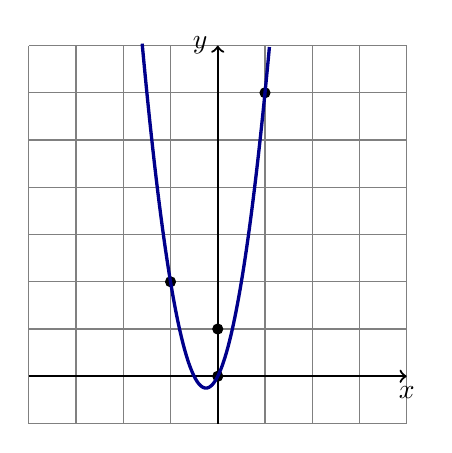
\begin{tikzpicture}[scale=0.6]
            \onslide<2->{ 
            \draw[gray,step=1cm,] (-4,-1) grid (4,7); 
            \draw[->,thick]  (-4,0) -- (4,0)  node [below] {$x$}; 
            \draw[->,thick]  (0,-1) -- (0,7) node [left] {$y$}; 
            \foreach \x/\y in  {-1/2,0/1,0/0,1/6}  \filldraw (\x,\y) circle (.3em); 
            }
            \onslide<3->{
            \draw [color=DarkBlue,very thick] plot[domain=-1.6:1.096,samples=200] (\x, {2*\x + 4*\x*\x }) ;
            }
    \end{tikzpicture}

    \end{center} 
    
\end{frame}







\begin{frame}\frametitle{Multiple Regression} 

    We can also consider least squares fitting for the form 
    \begin{equation*}
    z = c_0 + c_1 f_1  (x,y) + c_2 f _2 (x,y) + \cdots + c_k f _{k} (x,y).  
    \end{equation*}
    If functions $ f _{i}$ are known, this is another linear problem in the $c_i$ variables.

\vspace{12pt} 
\pause 
\Emph{Example: A Model of the Form $z=c_0 + c_1x + c_2y$} \\[6pt]
Consider the data in the table below. 

    \begin{center}
        \begin{tabular}{c|cccccc} 
            $ x$  & $-2$ & $-1$ & $0$ & $0$ & $1$ & $2$ 
            \\ \hline 
            $ y$ & $1$ &  $1$ & $-3$ & $-1$ & $1$ & $1
            $ 
            \\ \hline 
            $z$ & $2$ & $1$ & $1$ & $0$ & $-2$ & $-2$
        \end{tabular}
    \end{center}

    Determine the coefficients $c_1$ and $c_2$ for the surface $z = c_0 + c_1 x + c_2 y$ that best fits the data. 

\end{frame}



\begin{frame}\frametitle{Multiple Regression with $z=c_0 + c_1x + c_2y$}

    \begin{center}
        \begin{tabular}{c|cccccc} 
            $ x$  & $-2$ & $-1$ & $0$ & $0$ & $1$ & $2$ 
            \\ \hline 
            $ y$ & $1$ &  $1$ & $-3$ & $-1$ & $1$ & $1
            $ 
            \\ \hline 
            $z$ & $2$ & $1$ & $1$ & $0$ & $-2$ & $-2$
        \end{tabular}
    \end{center}
    \pause 
    Using the model $z=c_0 + c_1x + c_2y$, we obtain a matrix equation to represent our linear system. 
    $$A\vec x = \spalignmat{1 -2 1;1 -1 1;1 0 -3;1 0 -1;1 1 1;1 2 1 }\vec x = \spalignmat{2;1;1;0;-2;-2} = \vec b$$
    
\end{frame}



\begin{frame}\frametitle{Multiple Regression with $z=c_0 + c_1x + c_2y$}
    
    \pause 
    Constructing the normal equations, $A^TA \widehat x = A^T \vec b$, we obtain
    \pause 
    $$\spalignmat{6 0 0;0 10 0;0 0 14}\widehat x = \spalignmat{0;-11;-4}$$
    \pause
    This leads to the solution $$\widehat x = \spalignmat{0;-11/10;-2/7}$$
    Our model for our data is $z = -\frac{11}{10}x - \frac27 y$. 
    
\end{frame}




 \frame{\frametitle{Summary}

    \SummaryLine \vspace{4pt}
    \begin{itemize}\setlength{\itemsep}{8pt}

        \item the general linear model and least-squares to fit curves and surfaces to given data

    \end{itemize}
    
    \vspace{16pt}
    \pause 
    
    
}
